%%%%%%%%%%%%%%%%%%%%%%%%%%%%%%%%%%%%%%%%%
% Short Sectioned Assignment
% LaTeX Template
% Version 1.0 (5/5/12)
%
% This template has been downloaded from:
% http://www.LaTeXTemplates.com
%
% Original author:
% Frits Wenneker (http://www.howtotex.com)
%
% License:
% CC BY-NC-SA 3.0 (http://creativecommons.org/licenses/by-nc-sa/3.0/)
%
%%%%%%%%%%%%%%%%%%%%%%%%%%%%%%%%%%%%%%%%%

%----------------------------------------------------------------------------------------
%	PACKAGES AND OTHER DOCUMENT CONFIGURATIONS
%----------------------------------------------------------------------------------------

\documentclass[paper=a4, fontsize=11pt]{scrartcl} % A4 paper and 11pt font size

\usepackage[T1]{fontenc} % Use 8-bit encoding that has 256 glyphs
\usepackage{fourier} % Use the Adobe Utopia font for the document - comment this line to return to the LaTeX default
\usepackage[english]{babel} % English language/hyphenation
\usepackage{amsmath,amsfonts,amsthm} % Math packages

\usepackage{float} % position

\usepackage{lipsum} % Used for inserting dummy 'Lorem ipsum' text into the template

\usepackage{subfigure}
\usepackage{graphicx} % image in the same line

\usepackage{sectsty} % Allows customizing section commands
\allsectionsfont{\centering \normalfont\scshape} % Make all sections centered, the default font and small caps

\usepackage{fancyhdr} % Custom headers and footers
\pagestyle{fancyplain} % Makes all pages in the document conform to the custom headers and footers
\fancyhead{} % No page header - if you want one, create it in the same way as the footers below
\fancyfoot[L]{} % Empty left footer
\fancyfoot[C]{} % Empty center footer
\fancyfoot[R]{\thepage} % Page numbering for right footer
\renewcommand{\headrulewidth}{0pt} % Remove header underlines
\renewcommand{\footrulewidth}{0pt} % Remove footer underlines
\setlength{\headheight}{13.6pt} % Customize the height of the header

\numberwithin{equation}{section} % Number equations within sections (i.e. 1.1, 1.2, 2.1, 2.2 instead of 1, 2, 3, 4)
\numberwithin{figure}{section} % Number figures within sections (i.e. 1.1, 1.2, 2.1, 2.2 instead of 1, 2, 3, 4)
\numberwithin{table}{section} % Number tables within sections (i.e. 1.1, 1.2, 2.1, 2.2 instead of 1, 2, 3, 4)

\setlength\parindent{0pt} % Removes all indentation from paragraphs - comment this line for an assignment with lots of text


%----------------------------------------------------------------------------------------
%	pgfplots Config
%----------------------------------------------------------------------------------------

\usepackage{pgfplots}

%----------------------------------------------------------------------------------------
%	TIKZ Config
%----------------------------------------------------------------------------------------

\usepackage{tikz}
\usetikzlibrary{shapes,arrows, automata,positioning}

% shapes
\tikzstyle{startstop} = [rectangle, rounded corners, minimum width=3cm, minimum height=1cm,text centered, draw=black]
\tikzstyle{io} = [trapezium, trapezium left angle=70, trapezium right angle=110, minimum width=3cm, minimum height=1cm, text centered, draw=black]
\tikzstyle{process} = [rectangle, minimum width=3cm, minimum height=1cm, text centered, draw=black]
\tikzstyle{decision} = [diamond, aspect=3, text centered, draw=black]
\tikzstyle{point} = [coordinate]

% arrow
\tikzstyle{arrow} = [->,>=stealth]

% histogram
\pgfplotsset{
  compat=newest,
  xlabel near ticks,
  ylabel near ticks
}


%----------------------------------------------------------------------------------------
%	TITLE SECTION
%----------------------------------------------------------------------------------------

\newcommand{\horrule}[1]{\rule{\linewidth}{#1}} % Create horizontal rule command with 1 argument of height

\title{	
\normalfont \normalsize 
\textsc{South China University of Technology, School of Software Engineering} \\ [25pt] % Your university, school and/or department name(s)
\horrule{0.5pt} \\[0.4cm] % Thin top horizontal rule
\huge Computer Vision Assignment \#3 \\ % The assignment title
\horrule{2pt} \\[0.5cm] % Thick bottom horizontal rule
}

\author{Chen Mingjie, Lu Yonghao, Niu Zhe} % Your name

\date{\normalsize\today} % Today's date or a custom date

\begin{document}

\maketitle % Print the title

%----------------------------------------------------------------------------------------
%	PROBLEM 1
%----------------------------------------------------------------------------------------

\section{Abstract}
In this assignment, 
we evaluate the performance of the support vector machine based binary classifier
which utilizes features extracted by scale-invariant feature transform and clustered by k-means.
The evaluation is based on the Caltech 101 dataset. 
Results show this method has a great capability on binary classification of images.

\section{Introduction}
Nowadays, image classification has become a very hot topic. 
It refers to the task of categorizing a digital image into given classes. 
To do this, a general workflow is needed.
First, a dataset that contains the image data is needed, in which images should be labeled by their classes. 
The data set will then be divided into two major parts, the training set, and the test set.
The features of images from both training set and test set should be extracted before the classification.
This process is called feature extraction.
Feature extraction helps to reduce the calculations of the classifier and improve the accuracy, 
by means of generating lower dimension descriptions of images.
After feature extraction, the feature can be used as the input to the classifier to train and test the model.
The training set is used to train the classifier in the process showed in fig \ref{fig:proc:train}, 
\begin{figure}[H]
  \centering
  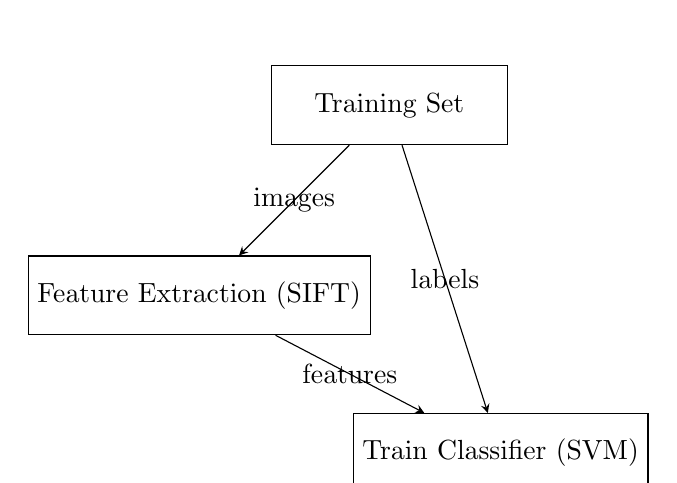
\begin{tikzpicture}[node distance=2cm, scale=0.5]
  \node[process](ts){Training Set};
  \node[process, below left of=ts, yshift=-1cm, xshift=-1cm](fe){Feature Extraction (SIFT)};
  \node[process, below right of=ts, yshift=-3cm](tc){Train Classifier (SVM)};
  \draw[arrow](ts) to node{images} (fe);
  \draw[arrow](fe) to node {features} (tc);
  \draw[arrow](ts) to node {labels} (tc);
  \end{tikzpicture}
  \caption{Training Process}
  \label{fig:proc:train}
\end{figure}
which will then be evaluated by the test set in the process showed in fig \ref{fig:proc:test}.

\begin{figure}[H]
\centering
  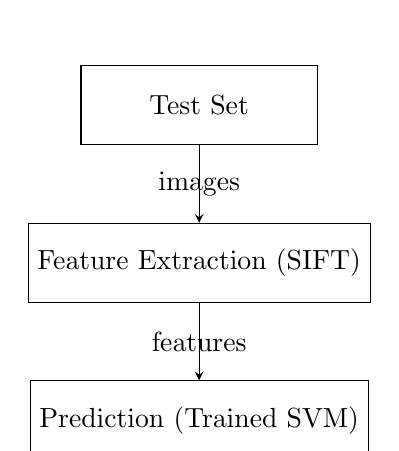
\begin{tikzpicture}[node distance=2cm]
  \node[process](ts){Test Set};
  \node[process, below of=ts](fe){Feature Extraction (SIFT)};
  \node[process, below of=fe](tc){Prediction (Trained SVM)};
  \draw[arrow](ts) to node{images} (fe);
  \draw[arrow](fe) to node {features} (tc);
  \end{tikzpicture}
  \caption{Test Process}
  \label{fig:proc:test} %% label for second subfigure
\end{figure}

In this assignment, we use scale-invariant feature transform (SIFT) as the feature extraction method and support vector machine (SVM) as the classifier.




\section{Feature Extraction: SIFT\cite{asgmt1}}
\subsection{Overview}
Scale-invariant feature transform (SIFT) is an algorithm to detects local features in images, 
which is both a keypoint detector and keypoint descriptor. 
It is proposed by David Lowe in 1999, and was patented by University of British Columbia.
The algorithm can be divided into four stages: 
Scale-space extreme detection, keypoint localization, orientation assignment and keypoint descriptor. 

\subsection{Scale-space Extreme Detection}
An image is first down-sampled and convolved with Gaussian filter.
$$
L(x, y, \sigma) = G(x, y, \sigma) * I(x, y)
$$
where 
$L$ is the blurred image, 
$G$ is the Gaussian Blur operator, 
$I$ is the original image, 
$x, y$ is the pixel location, 
$\sigma$ is the scale parameter, greater the value, greater the blur.
By using performing Gaussian filter with different scale parameter several times on different down-sampled images, new imaged are generated.
These images together with the original ones are then divided into different octaves according to the original down-sampled image.
The difference of images in the same octave will be taken after this. The difference is called Difference of Gaussian (DoG). 
Keypoints are then taken as the maxima or minima points of DoG $D(x, y, \sigma)$ that occur at different octave.
$$
D(x, y, \sigma) = L(x, y, k_i\sigma) - L(x, y, k_{i+1}\sigma)
$$
where $k_i$, $k_{i+1}$ is the scale parameter of convolved image $i$.

\subsection{Keypoint Localization}
The extreme points are usually too many, some of which are unstable.
Keypoint localization need to be performed to reject points that have low contrast or are poorly localized along an edge.
$$
D(\mathbf{x}) = D + \frac{\partial D }{\partial x}\mathbf{x} + \frac{1}{2}\mathbf{x^T}\frac{\partial ^ 2 D}{\partial \mathbf{x}^2}\mathbf{x}
$$
where $\mathbf{x} = (x, y, \sigma)^T$.
Minima or maxima point is located at 
$$
\hat{\mathbf{x}} = -\frac{\partial ^ 2 D^{-1}}{\partial \mathbf{x}^2}\frac{\partial D }{\partial \mathbf{x}}
$$
value of $D(\mathbf{x})$ must be large, $|D(\mathbf{x})| > threshold$.

\subsection{Orientation Assignment}
To generate a keypoint descriptor, each keypoint should be assigned a consistent orientation based on local image gradient directions. 
That will make the descriptor invariant to image rotation.
To perform all the computation in a scale-invariant manner, the scale $\sigma$ should be removed first from $L(x, y, \sigma)$.
Then the gradient magnitude $m(x, y)$ and $\theta(x, y)$ are computed as following:
$$
m(x, y) = \sqrt{(L(x+1, y) - L(x-1, y))^2 + (L(x, y+1) - L(x, y-1))^2}
$$
$$
\theta(x, y) = \arctan \frac{L(x, y+1) - L(x, y-1)}{L(x+1, y) - L(x- 1,y)}
$$

\subsubsection{Keypoint descriptor}
After the identification of keypoint and orientations assigned to them, a descriptor vector is ready to be calculated. 
A $16 \times 16$ window is set around the keypoint, which is then broken into sixteen $4 \times 4$ windows. 
In each $4 \times 4$ window, gradient magnitude and orientation are calculated. 360 degrees are divided into 8 bins, and each bin takes 45 degrees.
Results are put into the 8 bins, which form an 8-bin histogram.
There are sixteen $ 4 \times 4 $ sub-windows in the $16 \times 16$ window, which means, after calculation, a $16 \times 8$ dimensional vector will be generated as the feature vector.

\section{Feature Clustering: k-means}

\subsection{Overview}

\textbf{K-means} is a clustering method widely used in the unsupervised learning problem.
It clusters samples into a given number of classes so that each sample has a minimal distance to the center of the group it belongs.
In this assignment, we use it to convert our descriptors of key points of a picture to some highly abstracted features,
which then can be used as input of classifiers.
We call this process \textbf{feature clustering}.

\subsection{Lloyd's algorithm}
\textbf{Lloyd's algorithm} is a popular iterative technique used to calculate the clustering result of k-means. 
The main idea of the algorithm is to keep finding centers of new groups.
After finding new centers, all points in the space should be reassigned to the nearest new group based on the distance to its center.
As the member of the group changed by the reassignment, new center is generated.
The algorithm will keep running until the new centers and the old centers are approximately same.
The steps of this algorithm can be represented as following. Firstly, the \textbf{assignment step}:

$$
G_i^{(t)} = \left\{ x | D(x, c_i^{(t)}) \leq D(x, c_j^{(t)}) \ \forall j, 1 \leq j \leq K \right\}
$$

where $G_i^{(t)}$ is the group $i$ at time $t$, 
$D$ is the distance function (which can be Euclidean distance, Mahalanobis distance,  Hamming distance etc.),
$c_i$ is the center of group $i$ at time $t$, 
$K$ is the maximum number of clusters, which is set manually before the clustering,
and $x$ is the samples.The second step is called \textbf{update step}: 
$$
c_i^{(t+1)} = \frac{1}{|G_i^{(t)}|} \sum_{x_j \in G_i^{(t)}} x_j
$$
By repeating the two steps above until the centers of groups nearly stop changing, we will finally get a converged clustered model.

\subsection{Cluster Training and Feature Clustering}
We use the features extracted from all training images by SIFT to train our k-means cluster. 
The trained cluster will then be used to generate an input vector of the classifier SVM.
Specifically, when the features extracted from the key points in one single image is send to the cluster. 
The cluster will tell which classes do the key points belong to.
So the images, from both the training set and the test set, can be represented by the classes' information in the cluster rather than the raw SIFT features.
This helps to combine all key points in one single vector.
And we finally get normalized vectors of corresponding images, which will be used in following training and testing of the classifier.

\section{Classifier: Support Vector Machine}
\subsection{Overview} 
\textbf{Support Vector Machine (SVM)} is a popular classifier proposed first in 1963. 
It was only capable of the linear classification problem until 1992, a kernel trick was invented to deal with the nonlinear classification. 
In the following sections, we will first show how the linear classification works and then dive into the kernel trick.

\subsection{Linear Classification}
Suppose we have the linear separable data (fig \ref{fig:svm:lsd}). 
\begin{figure}[H]
\centering

\begin{tikzpicture}
\centering
\begin{axis}[
    axis lines=middle,
    xmin=0, xmax=6,
    ymin=0, ymax=6,
    xtick=\empty, ytick=\empty
]
\addplot [only marks, mark=-, mark size=3, semithick] table {
1 2
2 1
};
\addplot [only marks, mark=+, mark size=3, semithick] table {
2.5 2.5
3   3
};
\end{axis}
\end{tikzpicture}

\caption{The linear separable data}
\label{fig:svm:lsd}
\end{figure}

We want to choose a separation so that the margin between two groups can be maximized (fig \ref{fig::svm:mg}). 

\begin{figure}[H]
\centering

\begin{tikzpicture}
\centering
\begin{axis}[
    axis lines=middle,
    xmin=0, xmax=6,
    ymin=0, ymax=6,
    xtick=\empty, ytick=\empty
]
\addplot [only marks, mark=-, mark size=3, semithick] table {
1 2
2 1
};
\addplot [only marks, mark=+, mark size=3, semithick] table {
2.5 2.5
3 3
};

\addplot [domain=1.2:3.8, samples=4, color=red, thick] {-x+5};
\draw[<->, thick] (axis cs:1.55, 1.55) -- (axis cs:2.43, 2.43);
\addplot [domain=0.2:2.8, samples=4, color=red, thick] {-x+3};
\end{axis}
\end{tikzpicture}

\caption{Maximized margin}
\label{fig:svm:mg}
\end{figure}

To find the maximized margin, we should write the two line as linear equation. 
We want to define the boundaries of margin (i.e. the red lines) symmetrically. A way to do this is:
\begin{align}
\begin{split}
\mathbf{w}^T \mathbf{x} + b = \gamma \\
\mathbf{w}^T \mathbf{x} + b = -\gamma
\end{split}
\end{align}

The $\gamma$s are so cumbersome. 
As the $w$ and $b$ is arbitrary, we can just substitute $w$ with $\frac{w}{\gamma}$ and $b$ with $\frac{b}{\gamma}$, 
then we get:

\begin{align}
\begin{split}
\mathbf{w}^T \mathbf{x} + b = 1 \\
\mathbf{w}^T \mathbf{x} + b = -1
\end{split}
\end{align}

Now we have two boundaries. We can easily calculate the distance between them:

\begin{equation}
\mathrm{distance} = \frac{2}{||\mathbf{w}||}
\end{equation}

Our target is to maximized this distance in the premise that no sample is located in the margin, which means:

\begin{align}
\begin{split}
& \max_{\mathbf{w},\mathbf{b}} \ \frac{2}{||\mathbf{w}||} \\ 
s.t. \quad & \mathbf{w}^T \mathbf{x}_+ + b \geq 1, \forall \mathbf{x}_+ \in P\\
 & \mathbf{w}^T \mathbf{x}_- + b \leq -1 , \forall \mathbf{x}_- \in N
\end{split}
\label{eq:svm:t1}
\end{align}
Where $P$ is the set of all positive samples and $N$ is the set of all negative samples.
For mathematical convenience, we define $y$:

\begin{equation}
y_i = 
\begin{cases}  
+1,& \mathbf{x}_i \text{ is } \mathbf{x}_+\\
-1,& \mathbf{x}_i \text{ is } \mathbf{x}_-
\end{cases}
\end{equation}

And instead of trying to maximizing the $\frac{2}{||\mathbf{w}||} $, we minimize $\frac{||\mathbf{w}||^2}{2}$. 
The transforms above are carefully designed to make the later calculations easier. 
Now we can rewrite equation \ref{eq:svm:t1} in a simpler way:

\begin{align}
\begin{split}
& \min_{\mathbf{w},\mathbf{b}} \ \frac{||\mathbf{w}||^2}{2} \\ 
s.t. \quad & y_i(\mathbf{w}^T \mathbf{x}_i + b) \geq 1, \forall \mathbf{x}_i \in P \cup N \\ 
\end{split}
\end{align}

This is a convex optimal problem with inequality constraints, which can be solved by solving its Lagrange dual problem 
(Sadly, the Lagrange dual problem was not taught in the mathematical course of SSE, SCUT).
The dual problem can be represented as below:

\begin{align}
\begin{split}
L_D(\mathbf{\lambda}) = \inf_{\mathbf{w}, b} \ L_P(\mathbf{w}, b, \mathbf{\lambda}) =& \inf_{\mathbf{w}, b} \left( \frac{1}{2}||\mathbf{w}||^2 - \sum_i\lambda_i y_i(\mathbf{w}^T\mathbf{x}_i+b) + \sum_i\lambda_i \right)\\
&\max_\mathbf{\lambda} \ L_D(\mathbf{\lambda}) \\
\label{eq:svm:dl1}
\end{split}
\end{align}

Then we fix the $\mathbf{w}$ and $b$ to calculate the infimum. 
To do this, the partial derivative should be calculated and set to $0$:

\begin{align}
\begin{split}
\frac{\partial{L_P}}{\partial{\mathbf{w}}} =& \mathbf{w} - \sum_i\lambda_iy_i\mathbf{x}_i = 0 \\
\frac{\partial{L_P}}{\partial{b}} =& -\sum_i\lambda_iy_i = 0
\end{split}
\end{align}

Substitute $\mathbf{w}$ in equation \ref{eq:svm:dl1}, we get:

\begin{align}
\begin{split}
&\max_\mathbf{\lambda} \ L_D(\mathbf{\lambda}) = \sum_i\lambda_i - \frac{1}{2} \sum_i\sum_j\lambda_i\lambda_jy_iy_j\mathbf{x}_i^T\mathbf{x}_j\\
 &s.t. \ \sum_i\lambda_iy_i = 0, \lambda_i \geq 0, \forall i
\label{eq:svm:dl2}
\end{split}
\end{align}

$\mathbf{\lambda}$ can be calculated based on the algorithm called \textbf{sequential minimal optimization algorithm}. After training, the model can be used to do linear binary classification:

\begin{align}
\begin{split}
\mathbf{w}^T \mathbf{u} + b =  \left(\sum_i\lambda_iy_i\mathbf{x}_i^T\mathbf{u}\right) + b 
\end{split}
\end{align}

\section{Non-linear Classification}
For data inseparable, a \textbf{kernel function} to map the data to a higher dimension solves this problem. 
To do this, we rewrite the term $ \mathbf{x}_i^T\mathbf{x}_j $in equation \ref{eq:svm:dl2} to $K(\mathbf{x}_i^T, \mathbf{x}_j )$:

\begin{align}
\begin{split}
&\max_\mathbf{\lambda} \ L_D(\mathbf{\lambda}) = \sum_i\lambda_i - \frac{1}{2} \sum_i\sum_j\lambda_i\lambda_jy_iy_j K(\mathbf{x}_i^T, \mathbf{x}_j )\\
 &s.t. \ \sum_i\lambda_iy_i = 0, \lambda_i \geq 0, \forall i
\label{eq:svm:dl3}
\end{split}
\end{align}

where K is the kernel function, which first casts the samples, i.e. $\mathbf{x}_i $ and $ \mathbf{x}_j$, into higher dimension then calculate their dot product.
There are several common kernel functions such as polynomial kernel function: 
$$K(\mathbf{x}, \mathbf{y}) = (\mathbf{x}^T\mathbf{y} + 1) ^ p$$
radial basis function:
$$K(\mathbf{x}, \mathbf{y}) = e ^\frac{- ||\mathbf{x} -\mathbf{y}||^2}{2\sigma^2}$$
sigmoid function:
$$K(\mathbf{x}, \mathbf{y}) = \tanh(\kappa \mathbf{x}^T\mathbf{y} - \delta)$$

So far we get the kernel function, it helps us deal with the non-linear separable binary classification.
Image classification problem is generally non-linear separable problem, a kernel must be used when classify them.

\section{Data Set}

We use the \textbf{Caltech 101} dataset in this assignment. This dataset contain several classes of image. 
Images in this dataset are generally in size of $300 \times 200$ pixels. 
When training one model, 
we use 30 images in the target class as the positive samples and another 30 images picked randomly from other classes as negative samples.
Then we use 10 images different from the training images but still from the target class to test the model.
We use images from five classes to train five models independently.
The five classes are \textbf{anchor}, \textbf{butterfly}, \textbf{chair}, \textbf{cup}, and \textbf{motorbikes}.
Test result will be showed in the next section.



\section{Test Result}

\subsection{Overview}
We use the OpenCV library to perform these tests. All the codes are written in C++.
We trained five different models based on five training sets then used five test sets tested them. The tests have great result, which are showed in figure \ref{fig:res:1}

\begin{figure}[H]
\centering
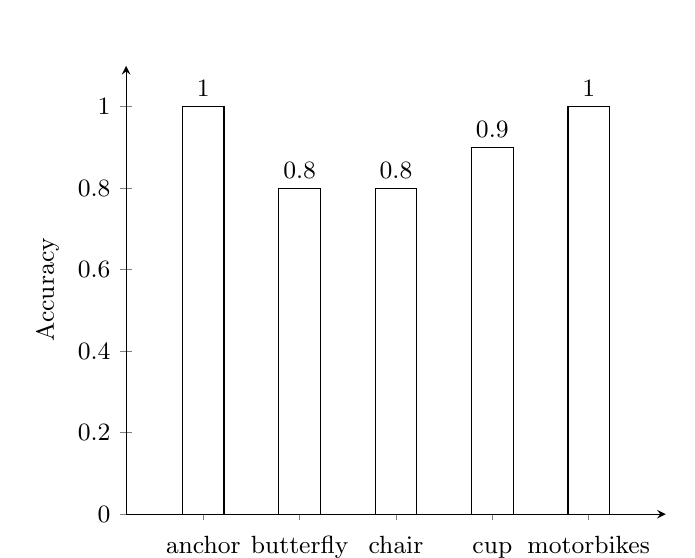
\begin{tikzpicture}[font=\small]
\begin{axis}[
    ybar,
    bar width=15pt,
    ylabel={Accuracy},
    ymin=0,
    ymax =1.1,
    xtick=data,
    axis x line=bottom,
    axis y line=left,
    enlarge x limits=0.2,
    symbolic x coords={anchor,butterfly,chair,cup,motorbikes},
    xticklabel style={anchor=base,yshift=-\baselineskip},
    nodes near coords={\pgfmathprintnumber\pgfplotspointmeta}
]
    \addplot[fill=white] coordinates {
    (anchor,        1.0)
    (butterfly,     0.8)
    (chair,         0.8)
    (cup,           0.9)
    (motorbikes,    1.0)
    };
\end{axis}
\end{tikzpicture}
\caption{Test Result}
\label{fig:res:1}
\end{figure}

%----------------------------------------------------------------------------------------
%	Anchor
%----------------------------------------------------------------------------------------

\subsection{Anchor}

\begin{table}[H]
\centering

\begin{tabular}{|l|l|}
\hline
\textbf{name}                 & \textbf{value} \\ \hline
number of class in clustering & 40             \\ \hline
kernel type                   & RBF            \\ \hline
$\gamma$ of kernel function   & 5              \\ \hline
maximum iterations            & 100            \\ \hline
terminate threshold           & 1e-6           \\ \hline
\end{tabular}
\caption{Parameters of the anchor model.}
\end{table}

The parameter of this model is listed as above.
This model gives a \textbf{1.0} accuracy to the test images of anchors.


%----------------------------------------------------------------------------------------
%	Butterfly
%----------------------------------------------------------------------------------------

\subsection{Butterfly}

\begin{table}[H]
\centering

\begin{tabular}{|l|l|}
\hline
\textbf{name}                 & \textbf{value} \\ \hline
number of class in clustering & 80             \\ \hline
kernel type                   & RBF            \\ \hline
$\gamma$ of kernel function   & 5              \\ \hline
maximum iterations            & 100            \\ \hline
terminate threshold           & 1e-6           \\ \hline
\end{tabular}
\caption{Parameters of the butterfly model.}
\end{table}

The parameter of this model is listed as above.
This model gives a \textbf{0.8} accuracy to the test images of butterflies.


%----------------------------------------------------------------------------------------
%	Chair
%----------------------------------------------------------------------------------------

\subsection{Chair}

\begin{table}[H]
\centering

\begin{tabular}{|l|l|}
\hline
\textbf{name}                 & \textbf{value} \\ \hline
number of class in clustering & 40             \\ \hline
kernel type                   & RBF            \\ \hline
$\gamma$ of kernel function   & 1              \\ \hline
maximum iterations            & 100            \\ \hline
terminate threshold           & 1e-6           \\ \hline
\end{tabular}
\caption{Parameters of the chair model.}
\end{table}

The parameter of this model is listed as above.
This model gives a \textbf{0.8} accuracy to the test images of chairs.

%----------------------------------------------------------------------------------------
%	Cup
%----------------------------------------------------------------------------------------

\subsection{Cup}

\begin{table}[H]
\centering

\begin{tabular}{|l|l|}
\hline
\textbf{name}                 & \textbf{value} \\ \hline
number of class in clustering & 40             \\ \hline
kernel type                   & RBF            \\ \hline
$\gamma$ of kernel function   & 5              \\ \hline
maximum iterations            & 100            \\ \hline
terminate threshold           & 1e-6           \\ \hline
\end{tabular}
\caption{Parameters of the cup model.}
\end{table}

The parameter of this model is listed as above.
This model gives a \textbf{0.9} accuracy to the test images of cups.

%----------------------------------------------------------------------------------------
%	Motorbike
%----------------------------------------------------------------------------------------

\subsection{Motorbike}

\begin{table}[H]
\centering

\begin{tabular}{|l|l|}
\hline
\textbf{name}                 & \textbf{value} \\ \hline
number of class in clustering & 40             \\ \hline
kernel type                   & RBF            \\ \hline
$\gamma$ of kernel function   & 5              \\ \hline
maximum iterations            & 100            \\ \hline
terminate threshold           & 1e-6           \\ \hline
\end{tabular}
\caption{Parameters of the motorbike model.}
\end{table}

The parameter of this model is listed as above.
This model gives a \textbf{1.0} accuracy to the test images of motorbikes.





%----------------------------------------------------------------------------------------
%	REF
%----------------------------------------------------------------------------------------


%----------------------------------------------------------------------------------------

\renewcommand\refname{Reference}
\bibliographystyle{unsrt}
\begin{thebibliography}{99}
\bibitem{asgmt1}
Niu Zhe, Computer Vision Assignment \#1.

\bibitem{kmeans}
Wikipedia, k-means clustering.

\bibitem{kmeans}
Wikipedia, support vector machine.

\bibitem{svm}
Patrick Henry Winston, MIT 6.034 Artificial Intelligence, Fall 2010, Lecture 16: Learning: Support Vector Machines.

% \bibitem{orb}
% Rublee E, Rabaud V, Konolige K, et al. ORB: An efficient alternative to SIFT or SURF[C]// IEEE International Conference on Computer Vision. IEEE, 2011:2564-2571.
\end{thebibliography}
\end{document}

\end{document}